\section{Proposed approach}
To accomplish our work we used a Convolutional Neural Network. This kind of model is now a days the most widely used for Image Recognition tasks. Many ways have been proposed to tackle the problem of stating similarity among different images, for example \cit{Schroff}{google}. Our solution is based on the idea of using directly convolutional layers to extract similarity, which is in our case expressed in terms of identity of people. In order to follow this idea, we used as input of our Convolutional Neural Network two gray scale images stacked one upon the other. Then, two dimensional Convolutional Layers filter those two levels images, transforming the initial input in tighter and thighter embeddings. The vector which comes from the last Convolutional Layer will contain an embedding of features which would naturally tell the relation between the two images in terms of similarity among identities of people appearing in those. Then the embedding of features is used as input of a Fully Connected Neural Network, which will, at the really end, output a number between 0 and 1, \ie the probability of having two photos who depict the same person.

\begin{figure}[t]
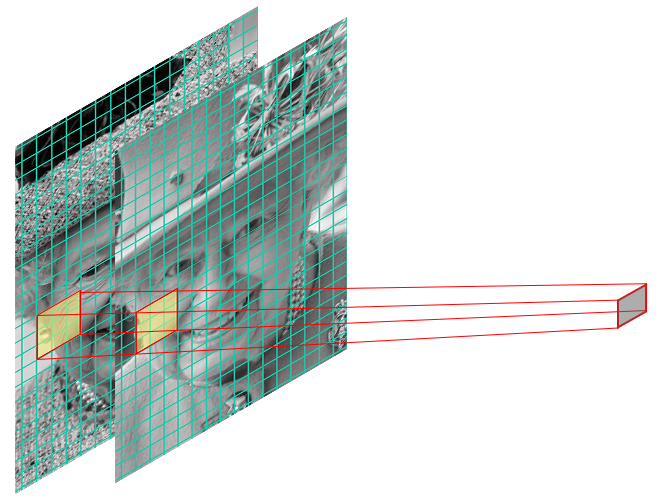
\includegraphics[width=0.8\linewidth]{images/stackedconvolution.png}
   \caption{Convolution between two stacked image. Large convolution filters can help to capture similiarities.}
\label{fig:long}
\label{fig:onecol}
\end{figure}

%-------------------------------------------------------------------------
\subsection{Mathematics}
We can consider training samples as i.i.d observations from a Bernoulli random variable. We want that our model approximates as well as possible this Bernoulli variable ($t_n$ can assume only values $0$ or $1$):
\begin{equation}
P(t_n = 1|x_n, \textbf{w}) = y(x_n)
\end{equation}
where $y(x_n)$ is the output of the convolutional neural network for the $n^{th}$ sample.
\\
We want to maximize the likelihood of getting the right ouput. To do so, we have to choose the vector of coefficients $\textbf{w}$ such that:
\begin{equation}
\argmax _{\textbf{w}} J(\textbf{w}) = \argmax _{\textbf{w}} \prod _n^N {y_n}^{t_n}(1-y_n)^{1-t_n}
\end{equation}
Passing to the negative log, we get the standard binary crossentropy:
\begin{equation}
\argmin _{\textbf{w}} J(\textbf{w}) = - \sum _{n=1}^{N}\ {\bigg [}t_{n}\log {y_n}+(1-t_{n})\log(1-{y_n}){\bigg ]}
\end{equation}

%-------------------------------------------------------------------------

\subsection{Model Selection}
The model selection has been one of the main challanges during our activity: we did not have other already existing works from which transfer the structure of the network, at least no other research product which was using the same approach to achieve the same goal. So first we decided to go for a Cross Validation among the possible models. Even if the amount of data that we managed to harvest (section 4) was enough to proceed with this idea, the methodology appeared to be computationally unfeasible. So we decided to go for a standerd validation approach. Of course we did not validate every possible model but instead we listed a set of fifteen networks of growing complexity. As a guideline for this ranking we have mainly considered \cit{Bengio}{hypsel}
To have the most unbiased estimate of the true error from our validation set, we randomly split the data into validation and training set before the actual validation procedure, and before any of the candidate network was trained and evaluated on the data.
When validating the various models, we used Adam Optimizer: this guaranteed to be free from the choice of the learning rate, removing one degree of freedom from our validation procedure.
The model resulting from our procedure is presented in Table 1
\\
\begin{table}[]
\label{tab:model}
\begin{center}
\begin{tabular}{l|l|l|l}
\thead{Layer} & \thead{Kernel} & \thead{Output shape} & \thead{\# of params} \\
\hline
Conv2D  & 3x3 (16) & (80, 80, 16)  & 304               \\
\hline
MaxPooling2D & 2x2 & (40, 40, 16)  & 0                \\
\hline
Dropout   & p=0.1 & (40, 40, 16)  & 0                \\

\hline
Conv2D    & 3x3 (16) & (40, 40, 16)  & 2320              \\
\hline
MaxPooling2D & 2x2 &(20, 20, 16)  & 0                \\
\hline
Dropout   & p=0.1 & (20, 20, 4)  & 0                \\

\hline
Conv2D   & 3x3 (16) & (20, 20, 16)  & 2320              \\
\hline
MaxPooling2D & 2x2 & (10, 10, 16)  & 0                \\
\hline
Dropout   & p=0.1 & (10, 10, 16)  & 0                \\

\hline
Conv2D    & 3x3 (16) & (10, 10, 16)  & 2320              \\

\hline
Flatten      & (1600)         & 0                \\

\hline
Dense   & 128 & (128)           & 204928          \\
\hline
Dropout  & p=0.1 & (128)           & 0                \\
\hline
Dense   & 128 & (128)           & 16512             \\
\hline
Dense   & 128 & (128)           & 16512                \\
\hline
Dense (softmax) & 2 & (2)            & 258              \\
\hline
\multicolumn{3}{l}{Total}   & 245474         
\end{tabular}
\end{center}
\caption{Structure of the network}
\end{table}
\\
All the models have been trained for twohundred epochs changing dinamically the training data: when the model started overfitting \ie when the training and test error were starting to be uncorrelated, we swapped to a different training set, sampled from the whole set of training samples. Every sampled chunck counted roughly fitythousand couples of images. This tecnique was on one hand necessary, because the whole dataset was not fitting on memory, and on the other hand turned out to be a powerful regularization tool.

%
%When placing figures in \LaTeX, it's almost always best to use
%\verb+\includegraphics+, and to specify the  figure width as a multiple of
%the line width as in the example below
%{\small\begin{verbatim}
%   \usepackage[dvips]{graphicx} ...
%   \includegraphics[width=0.8\linewidth]
%                   {myfile.eps}
%\end{verbatim}
%}

%------------------------------------------------------------------------
